\section{Overview}

This chapter presents the datasets used in the fire prediction task
(soil, climate, elevation, land cover and fire occurrence) and the main
visual explorations carried out on them. For each data source we
describe:
\begin{itemize}
    \item the original format and spatial/temporal coverage,
    \item the extraction and preprocessing steps applied to build the
          common $0.1^{\circ}$ grid over Algeria-Tunisia,
    \item the final features retained for modelling,
    \item a set of exploratory visualisations highlighting key spatial
          patterns and potential relationships with fire activity.
\end{itemize}

The goal is to provide a clear picture of what information is available
in each layer and how it behaves over the study area before moving to
the modelling stage.

% --------------------------------------------------------------------
% SOIL
% --------------------------------------------------------------------
\section{Soil data description and visualisation}
\section{Soil Dataset Description}

The soil dataset used in this study consists of \textbf{23,262 grid cells}
($0.1^{\circ}$ resolution) covering Algeria and Tunisia . Each row corresponds to a
regular grid-cell centroid (\texttt{x}, \texttt{y}) together with topsoil
(0--20\,cm) physical and chemical attributes extracted from the Harmonized World
Soil Database v2 (HWSD2). The total memory usage for the soil data is approximately \textbf{5.90 MB}. All features originate either from the D1 layer
(topsoil) or categorical summaries at the Soil Mapping Unit (SMU) level.

\subsection*{Spatial Columns}
\textbf{x, y} (\textit{longitude, latitude}) specify the centroid of each cell.
These coordinates enable spatial alignment with land cover, climate and
ignition datasets used in fire modelling \citep{Giglio2013}.

\subsection*{Identification Key}
\textbf{HWSD2\_SMU\_ID} uniquely identifies the soil mapping unit associated with
each cell. This ID links the grid to HWSD2 pedological information and ensures
consistent reproducibility \citep{FAO2021}.

\subsection*{Texture and Particle-Size Distribution}
\textbf{COARSE} (\,\%) represents the proportion of fragments $>2$\,mm, influencing
water retention and drying rates. High coarse content increases surface dryness
and ignition probability \citep{Prieto2019}.  
\textbf{SAND}, \textbf{SILT} and \textbf{CLAY} (\,\%) describe the granulometric
composition. Sandy soils drain rapidly and dry faster, whereas clay-rich soils
retain moisture and generally reduce fire susceptibility
\citep{Bowman2009,Saatchi2012}.  
\textbf{TEXTURE\_USDA} and \textbf{TEXTURE\_SOTER} provide categorical texture
classes (USDA and SOTER standards). Texture strongly regulates infiltration,
soil moisture availability and vegetation composition \citep{USDA2017,Batjes2016}.

\subsection*{Density and Structural Properties}
\textbf{BULK} (g\,cm$^{-3}$) measures dry soil density. Higher bulk density limits
root penetration and reduces water storage capacity \citep{Certini2005}.  
\textbf{REF\_BULK} is the expected bulk density estimated from pedotransfer
functions, used to detect compaction anomalies \citep{Reynolds2018}.

\subsection*{Organic Matter and Nutrients}
\textbf{ORG\_CARBON} (\%) represents organic carbon content, a driver of both
soil moisture retention and surface fuel accumulation \citep{DeGroot2009}.  
\textbf{TOTAL\_N} (\%) influences vegetation productivity and post-fire biomass
recovery \citep{Pausas2012}.  
\textbf{CN\_RATIO} (C:N) governs decomposition rates; high ratios slow down decay
and preserve surface litter, increasing flammability \citep{Fernandez2018}.

\subsection*{Chemical and Exchange Properties}
\textbf{PH\_WATER} indicates soil acidity. Extreme pH affects nutrient cycling
and decomposition, altering fuel loads \citep{Certini2005b}.  
\textbf{CEC\_SOIL}, \textbf{CEC\_CLAY} and \textbf{CEC\_EFF} (cmol\,kg$^{-1}$)
represent nutrient-holding capacity. High CEC improves water retention and thus
reduces fire proneness \citep{Brady2017,Jenny1941}.  
\textbf{TEB} (Total Exchangeable Bases) and \textbf{BSAT} (\%) describe soil
fertility; productive soils often accumulate more biomass, increasing available
fuel \citep{Archibald2013}.  
\textbf{ALUM\_SAT} (\%) and \textbf{ESP} (\%) capture aluminum and sodium
saturation. High ESP causes soil crusting and sparse vegetation, producing
patchy fire propagation patterns \citep{Qadir2014}.  
\textbf{TCARBON\_EQ} (total carbon equivalents) and \textbf{GYPSUM} (\%) indicate
soil development stage in arid systems. Gypsiferous and carbonate-rich soils
often host low vegetation cover and reduced fire intensity \citep{Herrero2009}.  
\textbf{ELEC\_COND} (dS\,m$^{-1}$) measures salinity; high salinity stresses
vegetation and correlates with lower fuel loads \citep{RuizSinoga2012}.

Overall, these variables collectively describe the soil moisture regime, nutrient
status, vegetation-support capacity and physical structure of the topsoil, all
of which are key environmental determinants of wildfire ignition and spread.


% --------------------------------------------------------------------
% CLIMATE
% --------------------------------------------------------------------
\section{Climate data description and visualisation}
\subsection{Data Description}\label{subsec:climate_description}

Climate variables were extracted from the \textit{WorldClim v2.1} monthly weather dataset at a spatial resolution of 5 arc-minutes (approximately 10 km). The study area covers Algeria and Tunisia, and the temporal scope spans the period 2020–2024. Three monthly climate variables were considered:
\begin{itemize}
    \item Total precipitation (\texttt{prec\_mm}, in millimeters),
    \item Maximum temperature (\texttt{tmax\_c}, in degrees Celsius),
    \item Minimum temperature (\texttt{tmin\_c}, in degrees Celsius).
\end{itemize}

Each variable was sampled on a common spatial grid using centroid-based extraction, yielding identical spatial coverage and temporal resolution. The resulting datasets have identical shapes:
\begin{itemize}
    \item Precipitation: $(1\,399\,320,\ 4)$,
    \item Maximum temperature: $(1\,399\,320,\ 4)$,
    \item Minimum temperature: $(1\,399\,320,\ 4)$.
\end{itemize}

Each dataset occupies approximately 42.7 MB in memory. All temperature values are expressed in degrees Celsius, ensuring physical interpretability and consistency across analyses.

\subsection{Data Visualization}\label{subsec:climate_visualization}

\subsubsection{Distribution Analysis}

Figure~\ref{fig:climate_histograms} presents the empirical distributions of precipitation, maximum temperature, and minimum temperature. Precipitation exhibits a highly right-skewed distribution, with a large concentration of low values and a long tail corresponding to intense rainfall events. This behavior is typical of semi-arid and Mediterranean climates, where dry conditions dominate most months.

Maximum and minimum temperatures display broader, multi-modal distributions reflecting strong seasonal variability. The separation between cold and warm regimes is clearly visible, with minimum temperatures spanning from sub-zero values to above $30^\circ$C, and maximum temperatures reaching nearly $50^\circ$C in extreme summer conditions.

\begin{figure}[H]
    \centering
    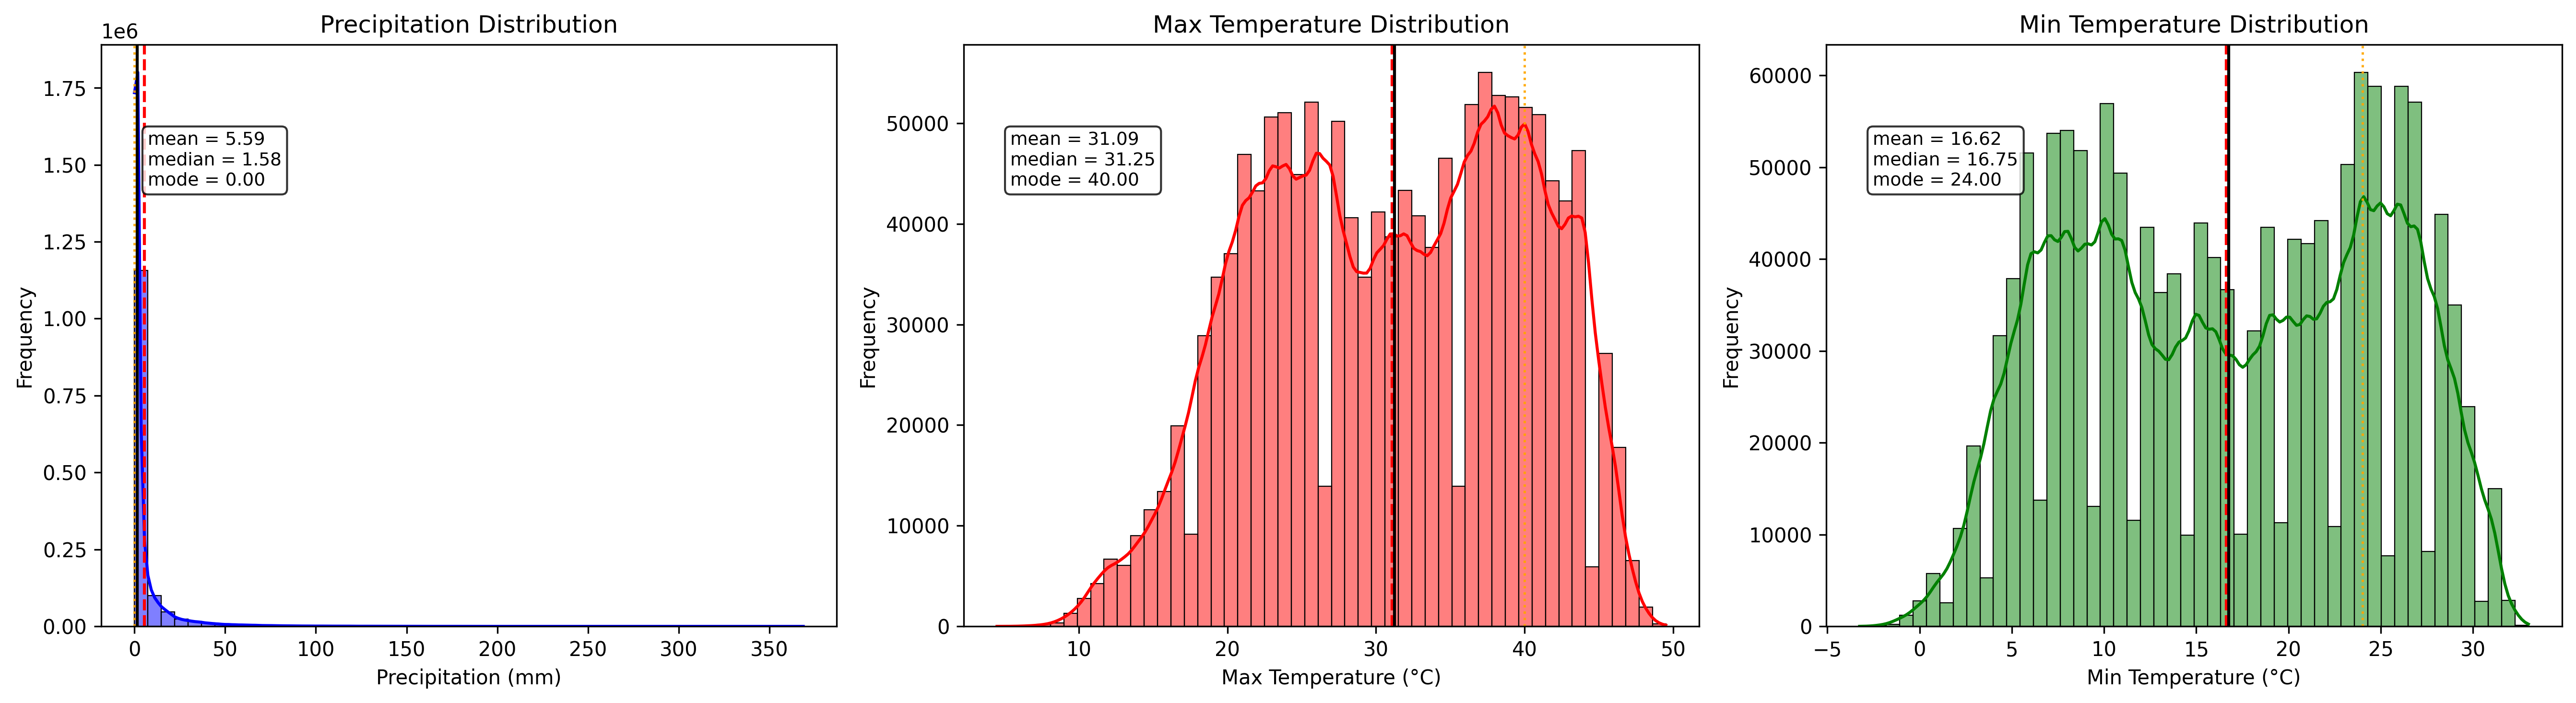
\includegraphics[width=0.95\linewidth]{images/Climate/climate_histograms_raw.png}
    \caption{Histograms of raw climate variables: precipitation, maximum temperature, and minimum temperature.}
    \label{fig:climate_histograms}
\end{figure}

Kernel Density Estimation (KDE) plots after imputation (Figure~\ref{fig:climate_kde}) confirm these observations. Precipitation remains strongly right-skewed, while temperature variables show smoother, multi-peaked density functions corresponding to seasonal cycles.

\begin{figure}[H]
    \centering
    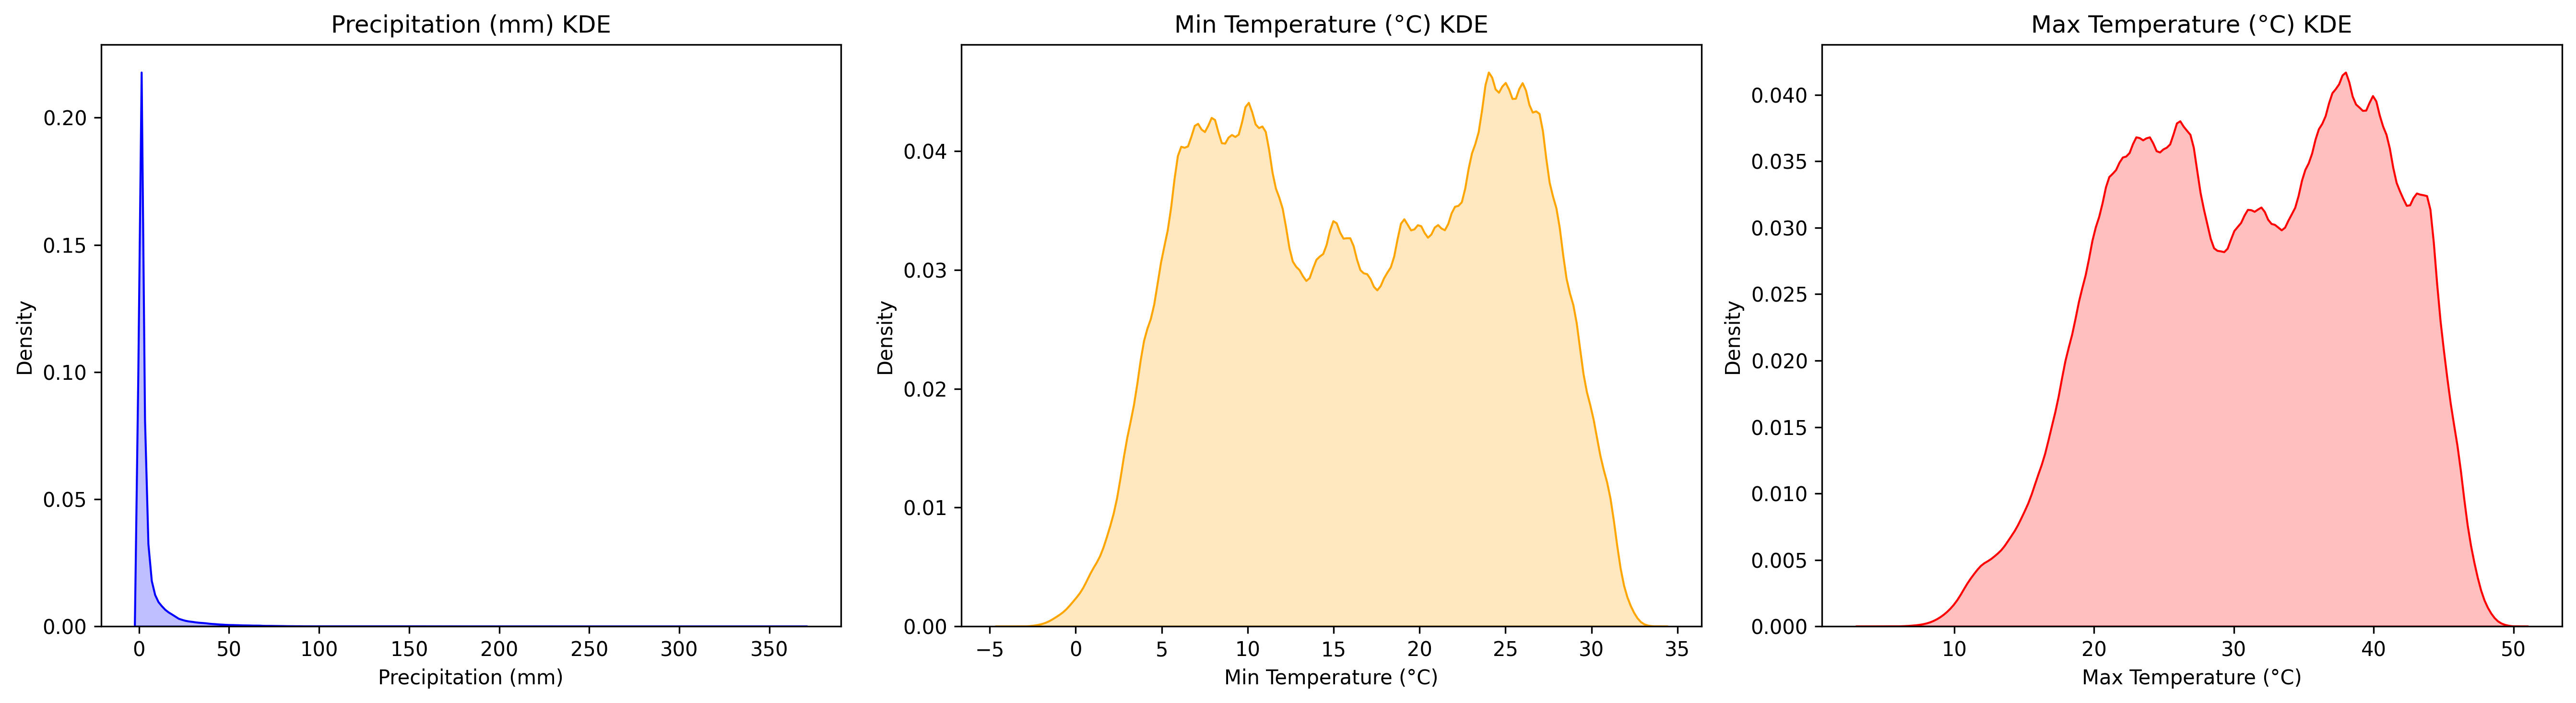
\includegraphics[width=0.95\linewidth]{images/Climate/climate_kde_imputed.png}
    \caption{Kernel density estimates of imputed climate variables.}
    \label{fig:climate_kde}
\end{figure}

\subsubsection{Normality Assessment}

Q--Q plots (Figure~\ref{fig:climate_qq}) indicate strong deviations from normality for precipitation, particularly in the upper quantiles, confirming the presence of heavy tails. Temperature variables exhibit more linear behavior in central quantiles but still deviate at the extremes, reflecting bounded physical processes and seasonal effects. These results indicate that no climate variable follows a Gaussian distribution, justifying the use of normalization or robust scaling rather than assumptions of normality.

\begin{figure}[H]
    \centering
    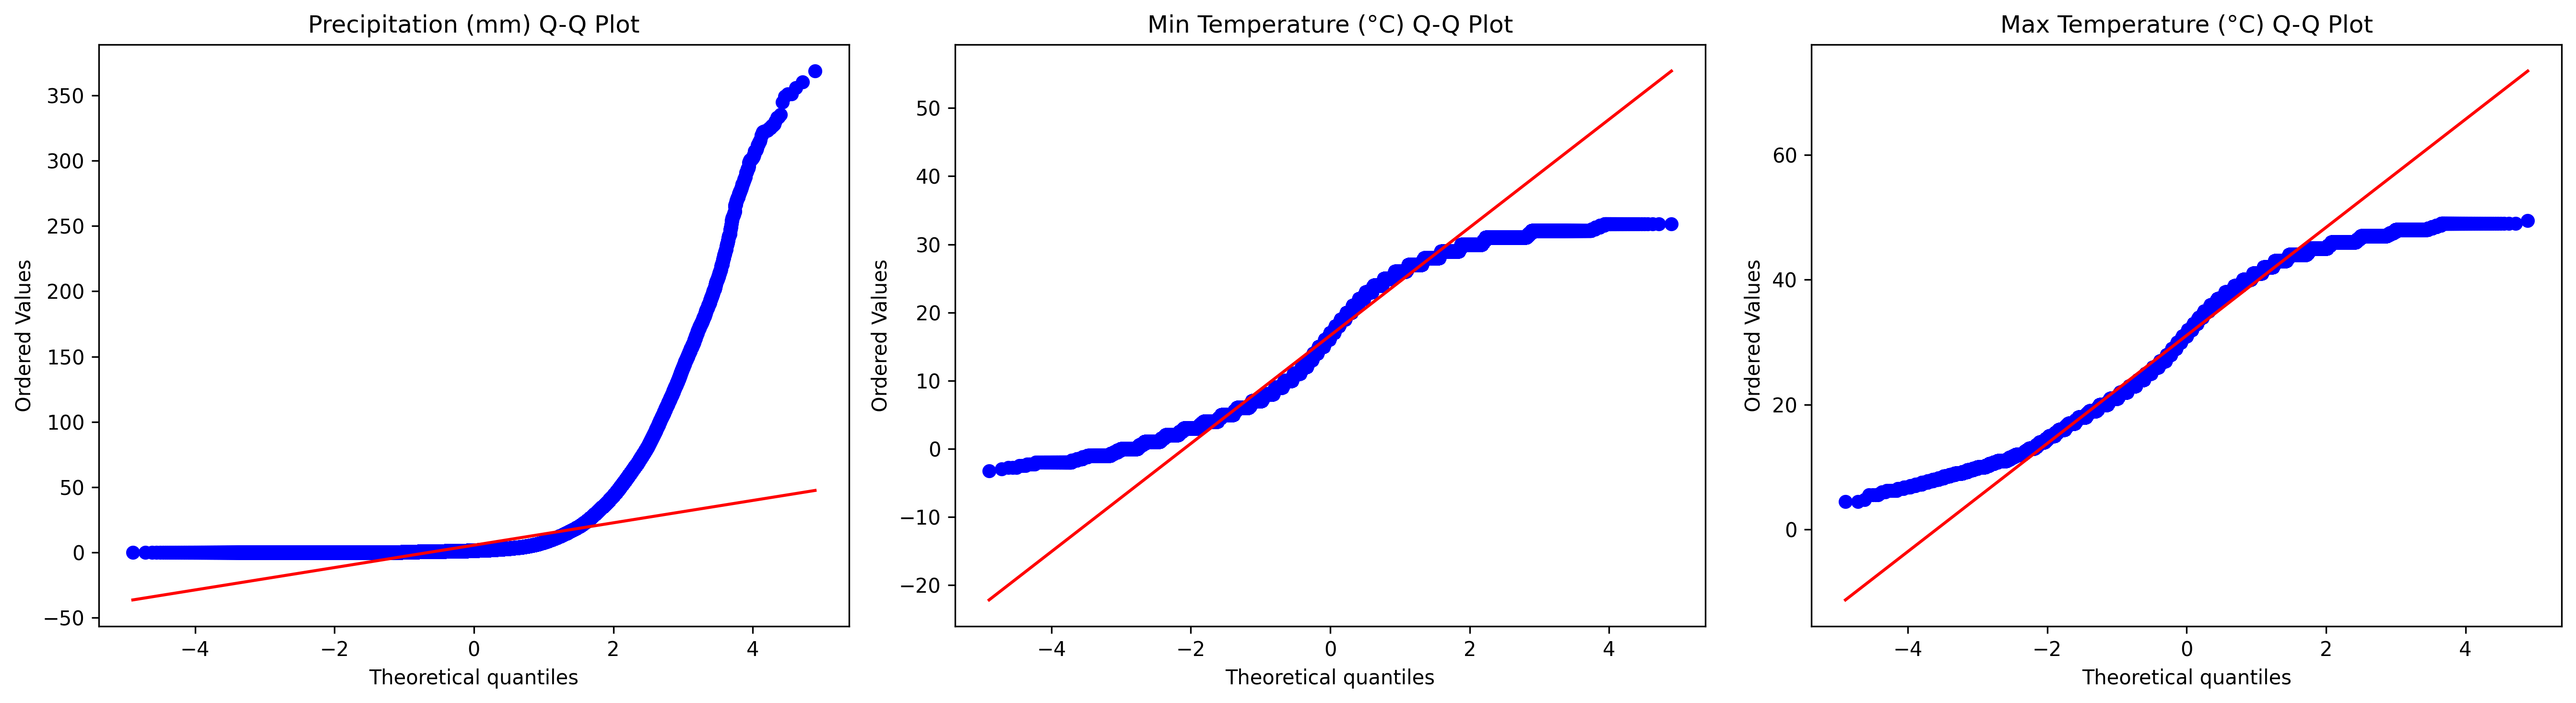
\includegraphics[width=0.95\linewidth]{images/Climate/climate_qq_plots_imputed.png}
    \caption{Q--Q plots for precipitation, minimum temperature, and maximum temperature after imputation.}
    \label{fig:climate_qq}
\end{figure}

\subsubsection{Spatial Patterns}

The figure in the Annex~\ref{annexe:climate-viz-summary} illustrates spatial heatmaps of mean climate conditions over the 2020–2024 period. Precipitation shows a strong north–south gradient, with wetter conditions in northern coastal and mountainous regions and extremely dry conditions in the Saharan south. Temperature maps display the inverse pattern: higher maximum and minimum temperatures dominate southern regions, while cooler conditions prevail at higher latitudes and elevations.

Monthly snapshot maps further highlight seasonal contrasts, particularly for January, where temperature gradients are most pronounced.


% --------------------------------------------------------------------
% ELEVATION / TOPOGRAPHY
% --------------------------------------------------------------------
\section{Elevation data description and visualisation}
This section details the analysis and statistical exploration of the extracted \textbf{Elevation Dataset} for the combined region of Algeria and Tunisia. The dataset is examined for data integrity, statistical properties, and spatial distribution.

\subsection{Data Loading and Integrity Check}

The analysis begins by loading the processed raster file using \texttt{rasterio}.

\begin{itemize}
    \item \textbf{No-Data Handling:} An integrity check was performed to identify and quantify the raster's no-data values (\texttt{nodata\_value}). These values, often representing areas outside the clipped boundary or sea level, were masked out during statistical calculations to ensure accurate topographical analysis.
\end{itemize}


\subsection{Descriptive Statistics and Visualisation}

Core statistics were computed on the valid elevation pixels to characterize the overall terrain:
    
    \begin{itemize}
        \item Mean Elevation: 538.327
        \item Median Elevation: 464.0
        \item Mode Elevation: 301
    \end{itemize}

The \textbf{Elevation Dataset}  was visualized to create a professional elevation map. The map utilizes a color scale to intuitively display elevation in meters.
 
\begin{figure}[H]
    \centering
    % Placeholder for the Elevation Map visualization
    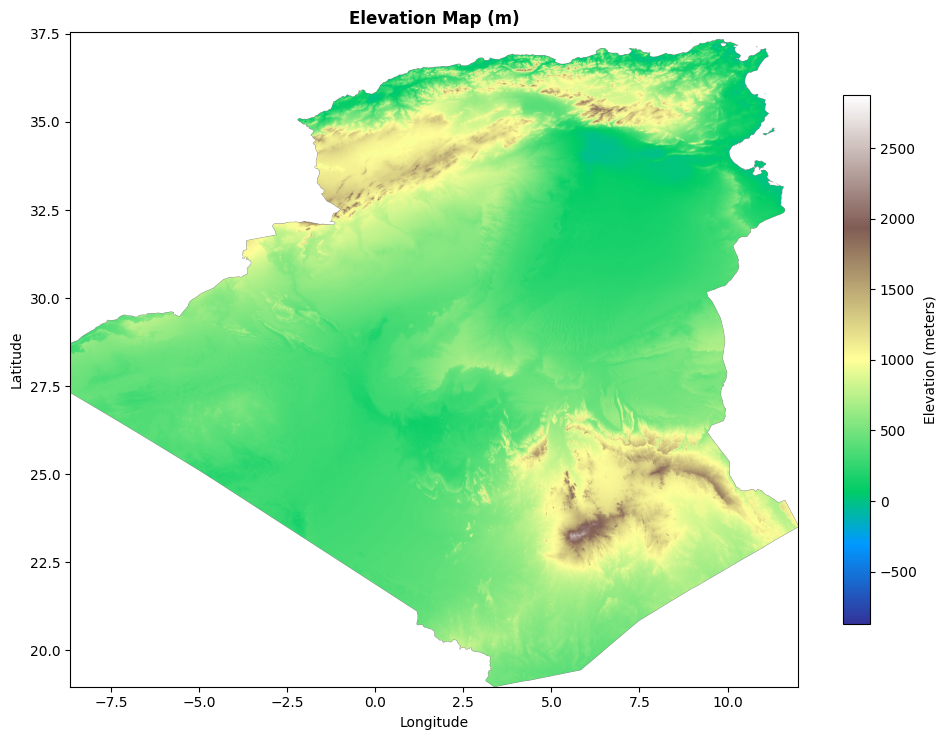
\includegraphics[width=0.5\textwidth]{images/Elevation/elevation map.png}
    \caption{Color-ramped visualization of the Elevation Dataset for the combined Algeria and Tunisia study area. The \texttt{terrain} color map illustrates the topographical gradient, ranging from low coastal plains to high inland mountains.}%
    \label{fig:elevation_map}
\end{figure}


% --------------------------------------------------------------------
% LAND COVER
% --------------------------------------------------------------------
\section{Land cover data description and visualisation}
Following the initial data integration, this section performs a detailed Exploratory Data Analysis (EDA) on the merged Land Cover dataset (\texttt{landcover\_combined.geojson}) to assess its structure, identify redundant features, and prepare the complex classification codes for modeling.

\subsection{Data Structure and Integrity}

The merged Land Cover GeoDataFrame (\texttt{landcover\_gdf}) was loaded and inspected for structural consistency.

\begin{itemize}
    \item \textbf{Data Counts:} The total number of unique features and the distinct values for the primary classification columns—$\texttt{lcccode}$ (Land Cover Classification Code) and $\texttt{gridcode}$—were tallied.
    \item \textbf{Redundancy Check:} An inspection for rows with duplicated $\texttt{id}$ values was performed. Although duplicates were found, the difference in associated geometry or attributes suggested they were not true feature duplicates, and the $\texttt{id}$ column was deemed non-essential for the model and slated for removal.
    \item \textbf{Missing Values:} A check across all columns confirmed the absence of any null or NaN values, indicating a complete and clean dataset structure following the initial GeoJSON conversion.
\end{itemize}

\textbf{Relationship between Classification Codes}
A key analysis focused on the relationship between $\texttt{gridcode}$ and $\texttt{lcccode}$. By checking unique pairs of these two columns, it was determined that they possess a one-to-one relationship. Consequently, $\texttt{gridcode}$ was identified as a redundant column that provides no additional information and is recommended for dropping during preprocessing.

 

\subsection{Initial Visualization and Area Analysis}

% \begin{figure} [H]
%     \centering
%     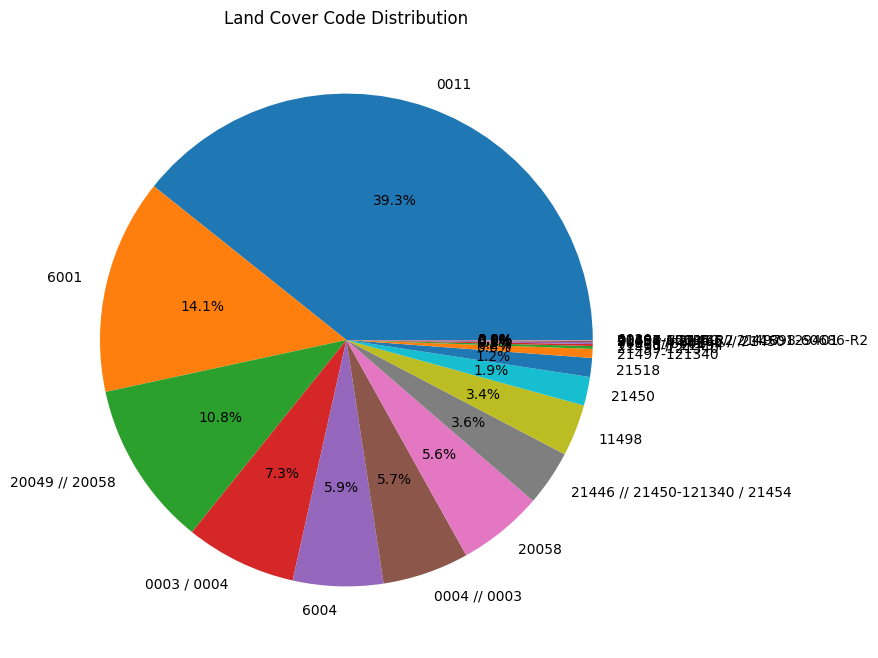
\includegraphics[width=0.8\textwidth]{images/LandCover/pie chart land cover distribution.png}
%     \caption{Pie chart illustrating the proportional distribution of Land Cover Codes ($\texttt{lcccode}$) across the combined study area.}
%     \label{fig:lcccode\_pie}
% \end{figure}

The distribution of land cover types was visualized to understand the regional composition:
\begin{itemize}    
    \item \textbf{Distribution Map:} The Land Cover Map was plotted, coloring polygons based on their $\texttt{lcccode}$ to visualize the spatial arrangement of classes.
    \begin{figure} [H]
    \centering
    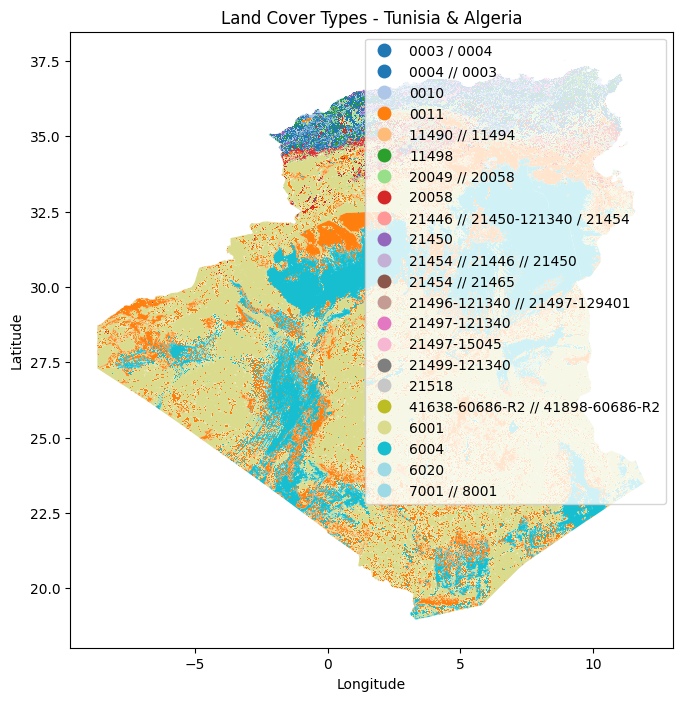
\includegraphics[width=0.5\textwidth]{images/LandCover/Land Cover Types - Algeria and Tunisia Merged.png}
    \caption{Geospatial visualization of the merged Land Cover Map, colored by the specific Land Cover Classification Code ($\texttt{lcccode}$).}%
    \label{fig:landcover_map}
\end{figure}

    % \item \textbf{Proportional Distribution:} A pie chart displayed the percentage distribution of each unique $\texttt{lcccode}$.
    \item \textbf{Area Analysis:} The geometric area of each polygon was calculated \\ ($\texttt{landcover\_gdf['area'] = \ldots geometry.area}$). A bar plot was generated showing the Total Area by Land Cover Code.


    \begin{figure} [H]
        \centering
        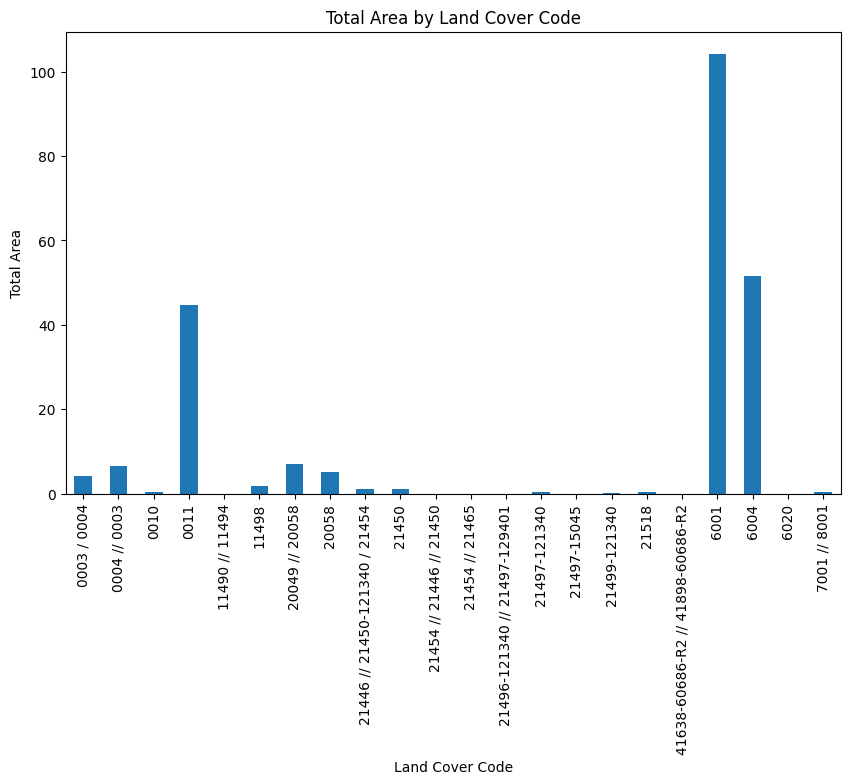
\includegraphics[width=0.6\textwidth]{images/LandCover/total area by lcc code bar chart.png}
        \caption{Total aggregated area (in square degrees) covered by each Land Cover Code in the combined dataset.}%
        \label{fig:lcccode_area}
    \end{figure}
\end{itemize}

 

% \subsection{Classification Code Harmonization}

% The raw $\texttt{lcccode}$ column contains complex codes (e.g., \texttt{7001 // 8001}) which represent mixed, uncertain, or transitional land cover types. The separator (\texttt{//}) indicates a mixture between the two classes (e.g., Shrubland and Bare/Sparse vegetation). To handle this complexity for machine learning, the following steps were taken:

% \textbf{Legend Integration}
% The official legend files (\texttt{globcover\_LCCS\_legend\_africa.xls} and \texttt{globcover\_legend.xls}) were loaded to establish a mapping between the numeric codes and descriptive labels.

% \begin{itemize}
%     \item The $\texttt{LCCCode}$ was mapped to its descriptive label ($\texttt{LCCOwnLabel}$) using a dictionary.
%     \item This process identified that certain codes were designated as ``Error'' in the $\texttt{LC}$ column of the legend, yet represented valid land cover types in the $\texttt{LCCOwnLabel}$ column (e.g., ``Closed forest''). This confirmed that these codes should be retained and mapped correctly.
% \end{itemize}

% \textbf{High-Level Mapping}
% Given the 22 unique $\texttt{lcccode}$ values in the dataset, a high-level, simplified mapping was created to aggregate these codes into fundamental categories (e.g., ``Forests,'' ``Bare lands,'' ``Croplands,'' ``Vegetation,'' etc.). 
% This step is crucial for reducing the complexity of the model's fire prediction.

% --------------------------------------------------------------------
% FIRE OCCURRENCE
% --------------------------------------------------------------------
\section{Fire data description and visualisation}
% \subsection{Data Loading and Inspection}
% The analysis began by loading the separate VIIRS (Visible Infrared Imaging Radiometer Suite) fire detection files for Algeria (\texttt{df\_fire\_dza}) and Tunisia (\texttt{df\_fire\_tun}).

% \begin{itemize}
%     \item \textbf{Initial Check:} Descriptive statistics \texttt{(describe())} were computed to understand the distribution, range, and central tendencies of numerical features like \texttt{frp} and brightness temperatures.
%     \item \textbf{Data Quality:} Inspection of data types, memory usage, and the percentage of missing values (\texttt{isnull().mean()}) confirmed data integrity and structure consistency across both datasets.
%     \item \textbf{Data Integration:} The two datasets were merged into a single GeoDataFrame, \texttt{df\_fire}, using the \texttt{pd.concat()} function, ready for combined regional analysis.
% \end{itemize}
\subsection{Data Loading and Inspection}

The analysis began by loading the datasets for Algeria (\texttt{df\_fire\_dza}) and Tunisia (\texttt{df\_fire\_tun}). An initial exploratory inspection was performed using descriptive statistics to assess the distribution and range of key numerical variables, including fire radiative power (\texttt{frp}) and brightness temperatures. Data quality was verified by examining data types, memory usage, and the proportion of missing values, confirming structural consistency and integrity across both datasets. Finally, the two datasets were merged using \texttt{pd.concat()} into a single GeoDataFrame (\texttt{df\_fire}), enabling unified regional analysis.


\subsection{Exploratory Data Analysis (EDA) and Visualization}

\begin{figure}[H]
    \centering
    
\includegraphics[width=0.45\textwidth]{\detokenize{images/Fire/frp values in map.png}}
    \caption{Geospatial distribution of fire events across Algeria and Tunisia. Points are colored by Fire Radiative Power (FRP), highlighting areas of highest fire intensity.}\label{fig:fire_spatial_map}
\end{figure}

The geospatial distribution of fire events was visualized using a scatter plot of \texttt{longitude} vs.\ \texttt{latitude}, with the color intensity mapped to \texttt{frp}. This visualization is essential for identifying fire clusters and high-intensity regions across the combined study area.
As shown in the map, the majority of fire points are concentrated in the northern regions, reflecting higher vegetation density and more favorable climatic conditions for fire occurrence compared to the arid southern areas


% \begin{figure} [H]
%     \centering
%     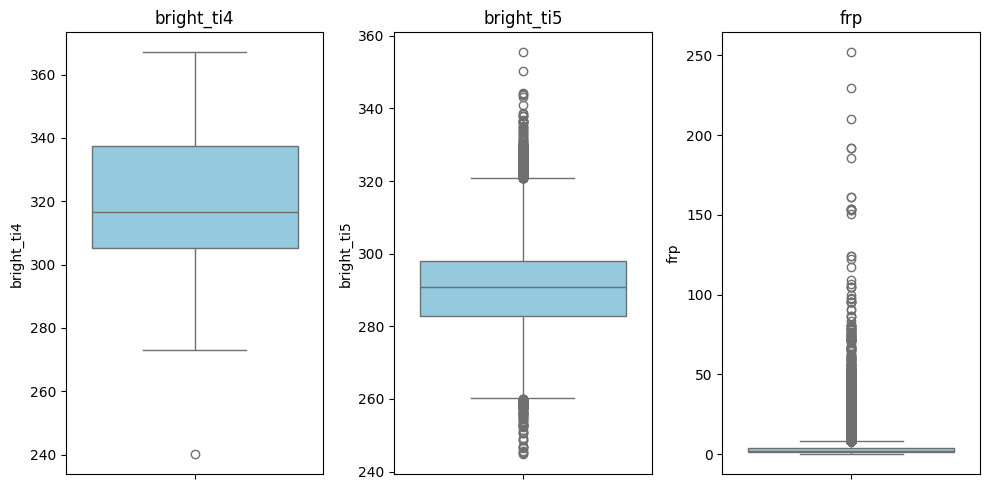
\includegraphics[width=0.8\textwidth]{images/Fire/boxplots.png}
%     \caption{Boxplots displaying the distribution of fire intensity metrics (\texttt{bright\_ti4, bright\_ti5, frp}), clearly illustrating the presence of extreme outliers (high-power fires) above the main interquartile range.}
%     \label{fig:boxplots}
% \end{figure}

% Boxplots (Figure \ref{fig:boxplots}) further confirmed the presence of significant outliers in the fire intensity metric $\texttt{bright\_ti5}$ and $\texttt{frp}$), due to the presence of extremely hot and large fire events.



% (Optional)
% --------------------------------------------------------------------
% SUMMARY
% --------------------------------------------------------------------
\section{Summary}

Across all datasets, we obtain a harmonised $0.1^{\circ}$ grid where each
cell is described by soil, climate, topography, land cover and fire
occurrence variables. The exploratory maps and distributions presented
in this chapter reveal the main gradients (e.g.\ climatic aridity,
vegetation cover, soil texture) that will later be exploited as
predictors in the supervised and unsupervised learning experiments.
